\apendice{Especificación de Requisitos}

\section{Introducción}
En este apéndice se detallan los requisitos del proyecto, como los funcionales y no funcionales. La finalidad es hacer de intermediario entre el cliente y los programadores, con el objetivo de ayudar a entender, comprender y analizar la aplicación. 

\section{Objetivos generales}
Este trabajo final de grado focaliza la aplicación mediante dos puntos de vista totalmente diferentes, dependiendo de las situaciones futuras a las que se someta la aplicación, siempre englobado en el marco de que es un producto que nos encarga la universidad de Burgos, como cliente final.

\begin{itemize}
	\item Colección de videojuegos. Tener una gran cantidad de estos mismos, para lograr sacar un rendimiento económico gracias a lo publicidad, por lo que es necesario que la aplicación tenga una gran repercusión en el mercado. Esto implica que a futuro se debe de hacer una inversión en publicidad y \emph{marketing}.
	\item \emph{Porfolio} \cite{wiki:portafolio} o escaparate con el que mostrar las capacidades técnicas, herramientas usadas o lenguajes de programación aprendidos, ante los equipos de recursos humanos en las empresas, llegado el momento de tener que buscar trabajo. 
\end{itemize}

\section{Catalogo de requisitos}
A continuación se numeran los requisitos del proyecto extraídos de los generales.

\subsection{Requisitos funcionles}
Por cada uno de los requisitos funcionales, va a tener una correlación con la pantalla en la que se da la operatividad del mismo, excepto en los casos en las que este requerimiento abarca varias ventanas.

Algunos de los requisitos funcionales, en el momento de ser tratados con el cliente, tuvieron apoyo de unos \emph{sketch} o bocetos conceptuales, con el fin de dar soporte, ayudar a comprender y facilitar la comunicación cliente - analista. Como podemos ver en la imagen~\ref{fig:bocetolog}, o en el apéndice de diseño~\pageref{diseño}.

\begin{figure}[H]
	\centering
	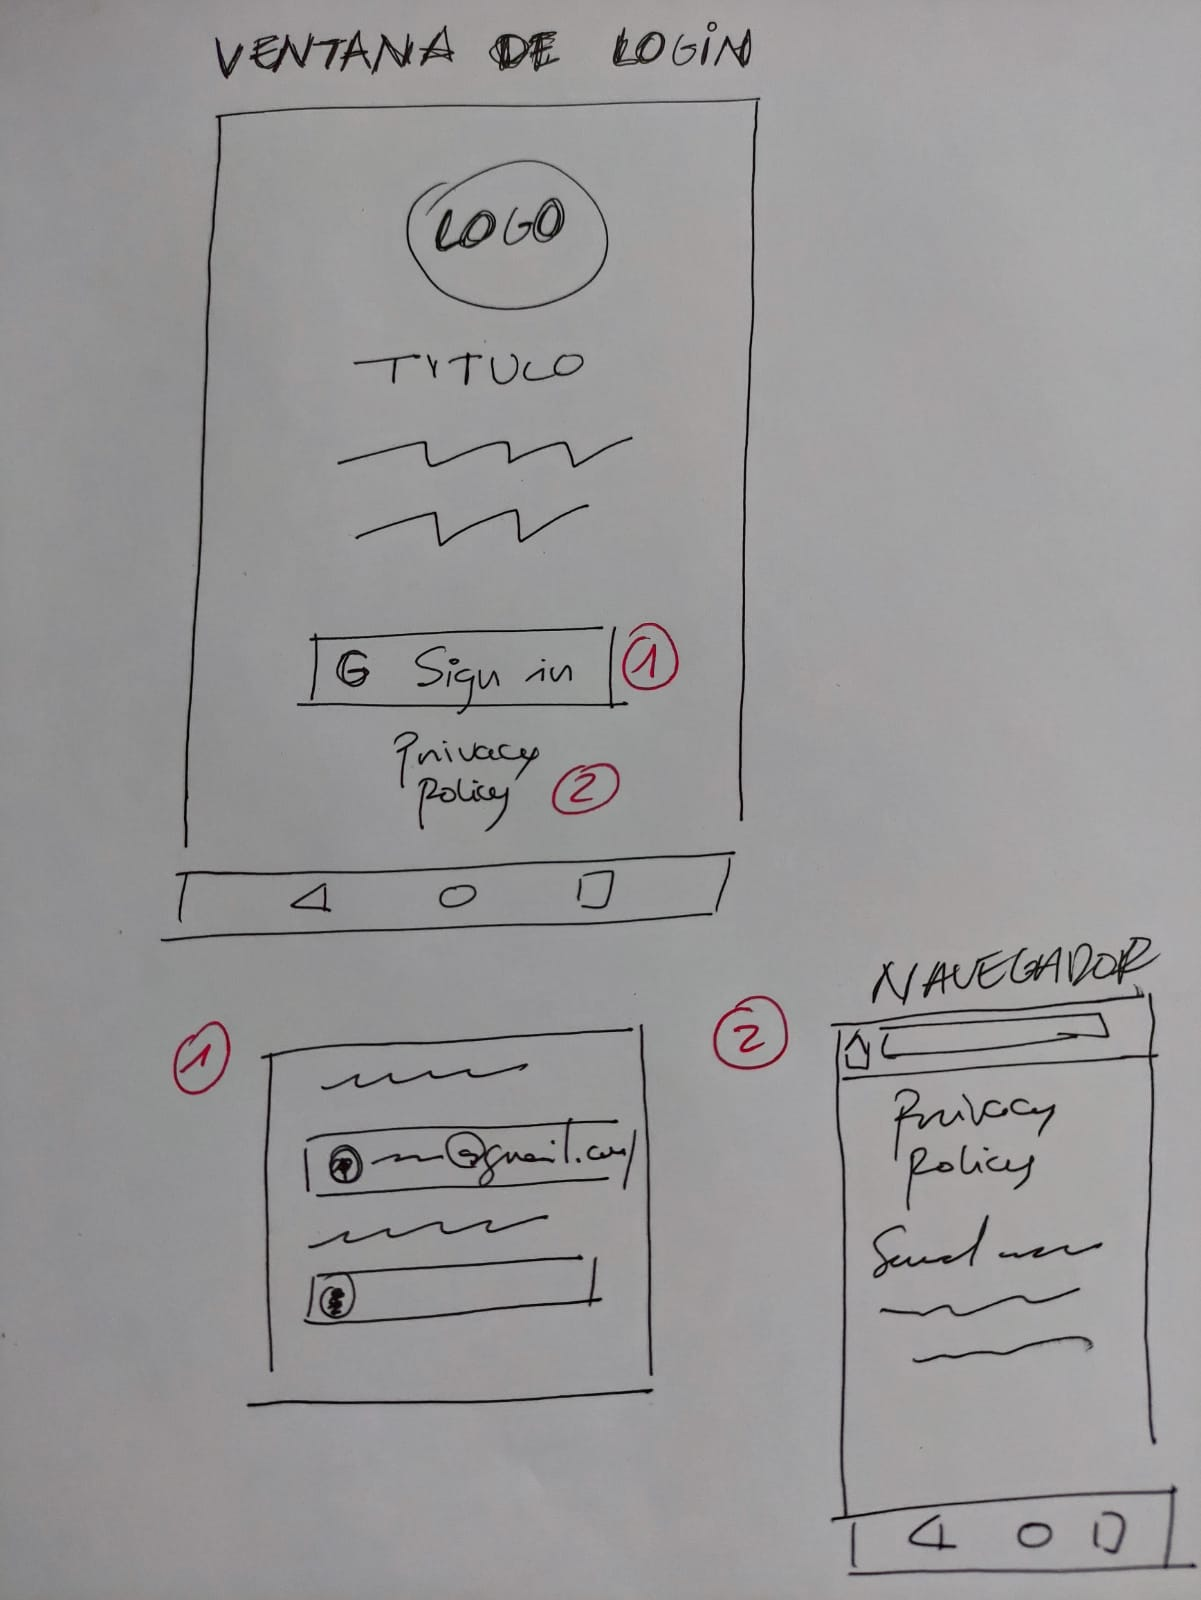
\includegraphics[height=0.9\textwidth]{requisitos/bocetolog.jpeg}
	\caption{Boceto sing in}\label{fig:bocetolog}
\end{figure}

\begin{itemize}
\tightlist
	%%INICIO DE LA SESIÓN
	\item \textbf{RF-1 Ventana de \emph{sign in:}~\ref{fig:loginpage}} La aplicación tiene que contener una ventana principal con la que los usuarios puedan iniciar la sesión, con el fin de tener servicios en la nube.
	
	\begin{itemize}
	\tightlist
	\item \textbf{RF-1.1 Botón de inicio sesión:} Mediante un elemento clickable se debe de tener acceso a un formulario para poder entrar mediante la cuenta de \emph{Google}.
	\item \textbf{RF-1.2 Consultar la política de privacidad:} Un enlace en el que se pueda mostrar todo lo referente a la política de privacidad.
	\item \textbf{RF-1.3 Cerrar sesión:} ser capaz de salir de la aplicación \emph{sign out}, desde cualquier ventana.
	\end{itemize}
	
	%% MENÚ DE NAVEGACIÓN PERMANENTE DURANTE LA EJECUCIÓN
	\item \textbf{RF-2 Menú de navegación:~\ref{fig:menuhome}} Se considera necesario tener la capacidad de navegar de una parte a otra dentro de la aplicación, sin tener que pasar entre ventanas, mediante un menú. 
	
	\begin{itemize}
		\tightlist
		\item \textbf{RF-2.1 Mostrar el menú lateral} el usuario debe poder entrar al menú mediante un \emph{scroll lateral}.
		\item \textbf{RF-2.2 Navegar:} la capacidad de navegar entre las diferentes ventanas que ofrece la aplicación.
		\item \textbf{RF-2.3 Integración con el RF-1.3:} Para que se disponga la salida en cualquier momento de la aplicación es necesario incluir en el menú, los datos de usuario con la capacidad de salir.
	\end{itemize}

	%% ALGUNOS DE LOS AJUSTES DEBEN DE SER SELECCIONABLES
	\item \textbf{RF-3 Configurar app~\ref{fig:settingspage}} la aplicación tiene que ser capad de gestionar algunas de las diferentes capacidades del producto, que el usuario desee.
	
	\begin{itemize}
		\tightlist
		\item \textbf{RF-3.1 Opción \emph{dark mode}:} la aplicación tiene que ser capada de cambiar el color del sistema, para ahorrar batería o para mejorar el contraste.
		\item \textbf{RF-3.2 Opciónes del juego snake:} algunas de las opciones de este juego deben de ser controlables desde el apartado de ajustes.
	\end{itemize}
	
	%% INFORMACIÓN RELEVANTE SOBRE EL CREADOR DE LA APLICACIÓN
	\item \textbf{RF-4 Ventana de \emph{about}~\ref{fig:aboutpage}} mostrar información sobre el creador de la aplicación.
	
	\begin{itemize}
		\tightlist
		\item \textbf{RF-4.1 Mostrar carousel imagenes:} enseñar al usuario fotografías de los lenguajes de programación que el creador de la aplicación conoce.
		\item \textbf{RF-4.2 Consultar mediante \emph{iconbuttons}:} unos botones que redirijan a contenido relevante del creador.
	\end{itemize}
	
	%% PUBLICIDAD INTEGRADA
	\item \textbf{RF-5 Publicidad integrada} la aplicación debe de ser capad de mostrar anuncios.
	
	\begin{itemize}
		\tightlist
		\item \textbf{RF-5.1 Mostrar \emph{banner}:} mostrar en el \emph{footer} un contenedor de anuncios, proporcionados estos por Google.
		\item \textbf{RF-5.2 Continuar Snake:} el usuario tiene que ser capad de ver un video, como recompensa, continuar en la partida. 
	\end{itemize}

	%% JUEGO DEL SNAKE
	\item \textbf{RF-6 Juego del snake \ref{fig:snakepage}:} el usuario tiene que ser capad de jugar a este juego.
	
	\begin{itemize}
		\tightlist
		\item \textbf{RF-6.1 Jugar snake:} la aplicación tiene que ser capad de trabajar con los choques que se producen, con la comida, pared, bloques, o tuberías.
		\item \textbf{RF-6.2 Mostrar la puntuación:} la app tiene que ser capad de mostrar la puntuación que lleva en la partida.
		\item \textbf{RF-6.3 Compartir la puntuación:} el jugador tiene que ser capad de subir la puntuación una vez termine la partida. Siempre y cuando esta sea mejor a otra anterior.
		\item \textbf{RF-6.4 Mostrar el ranking:} el usuario tiene que ser capad de ver la puntuación del resto de jugadores, así como la que ha logrado.
	\end{itemize}

	%% JUEGO DEL CUATRO EN RAYA
	\item \textbf{RF-7 Juego del cuatro en raya \ref{fig:cuatromenu}:} el usuario tiene que ser capad de jugar a este juego.
	
	\begin{itemize}
		\tightlist
		\item \textbf{RF-7.1 Mostrar menú juego:} la app tiene que ser capad de enseñar un menú intermedio con el fin de poder elegir entre invitar o unirse.
		\item \textbf{RF-7.2 Invitar:} el usuario tiene que ser capad de invitar a otro jugador, compartiendo una clave de acceso a la partida. Tiene que haber un botón que ayude a hacer esta tarea.
		\item \textbf{RF-7.3 Unirse:} el usuario mediante un formulario debe de ser capad de ingresar la clave de acceso de la parida.
		\item \textbf{RF-7.4 Jugar cuatro en raya:} la aplicación tiene que ser capad de controlar los diferentes eventos se producen durante la partida, como pueden ser, sorteo de inicio, ficha no válida, formación del cuatro en raya, advertir de quien gana.
		\item \textbf{RF-7.5 Hablar mediante chat:} el usuario tiene que tener la capacidad de mandar mensajes cortos, de no más de 15 caracteres. Después de remitir el mensaje, se tiene que bloquear esta opción durante 10 segundos, para no sobrescribir otros mensajes o que se sature el juego.
	\end{itemize}

\end{itemize}

\subsection{Requisitos no funcionles}
\begin{itemize}
	\tightlist
	%%INICIO DE LA SESIÓN
	\item \textbf{RNF-1 Rendimiento:} la capacidad de dar una calidad de producto homogénea, no se debe ver menguada por tiempos de carga, cuelgues en el sistema o cualquier problema / incidencia que lastre el desempeño del producto.
	\item \textbf{RNF-2 Seguridad:} ofrecer la aplicación desde la \emph{Store}, ya que esta tiene soporte integrado de antivirus. Lo que una garantía de confianza. Ninguno de los datos deben de ser ofrecidos a terceros, exceptuando a Google. 
	
	Mediante una cifrado de extremo a extremo (SHA-1~\cite{wiki:sha1}) se realizaran las comunicaciones con \emph{Firebase cloud}.
	
	\item \textbf{RNF-3 Escalabilidad:} todo el sistema tiene que ser escalable dependiendo del número de usuarios simultáneos que estén usando la app.
	\item \textbf{RNF-4 Usabilidad:} interfaces como las interacciones con el usuario, tienen que ser lo más amigables posibles. (\emph{responsive})
	\item \textbf{RNF-5 Disponibilidad:} la aplicación tiene que estar operativa en cualquier momento, así como garantizar una frecuencia de actualizaciones periódica.
	\item \textbf{RNF-6 Plataforma:} dirigido a dispositivos con el sistema operativo Android, desde la versión 10.0 Lollipop.
\end{itemize}

\section{Especificación de requisitos}
En este apartado se muestran los diagramas de casos de uso, con una breve descripción.

\subsection{Actores}
Solo tenemos un tipo de actor que puede interactuar con la aplicación, que es el usuario estándar. Este será capad de ver todo el contenido que tiene asociado a su cuenta.

Como apreciación, los desarrolladores tendrán acceso al \emph{backend}, donde se puede gestionar la plataforma y la tienda. Pero no es un usuario final de la aplicación, por lo que quedan excluidos del diagrama de casos de uso. Ya que esto es algo inherente a su cargo.

\subsection{Diagrama de casos de uso}
\begin{figure}[H]
	\centering
	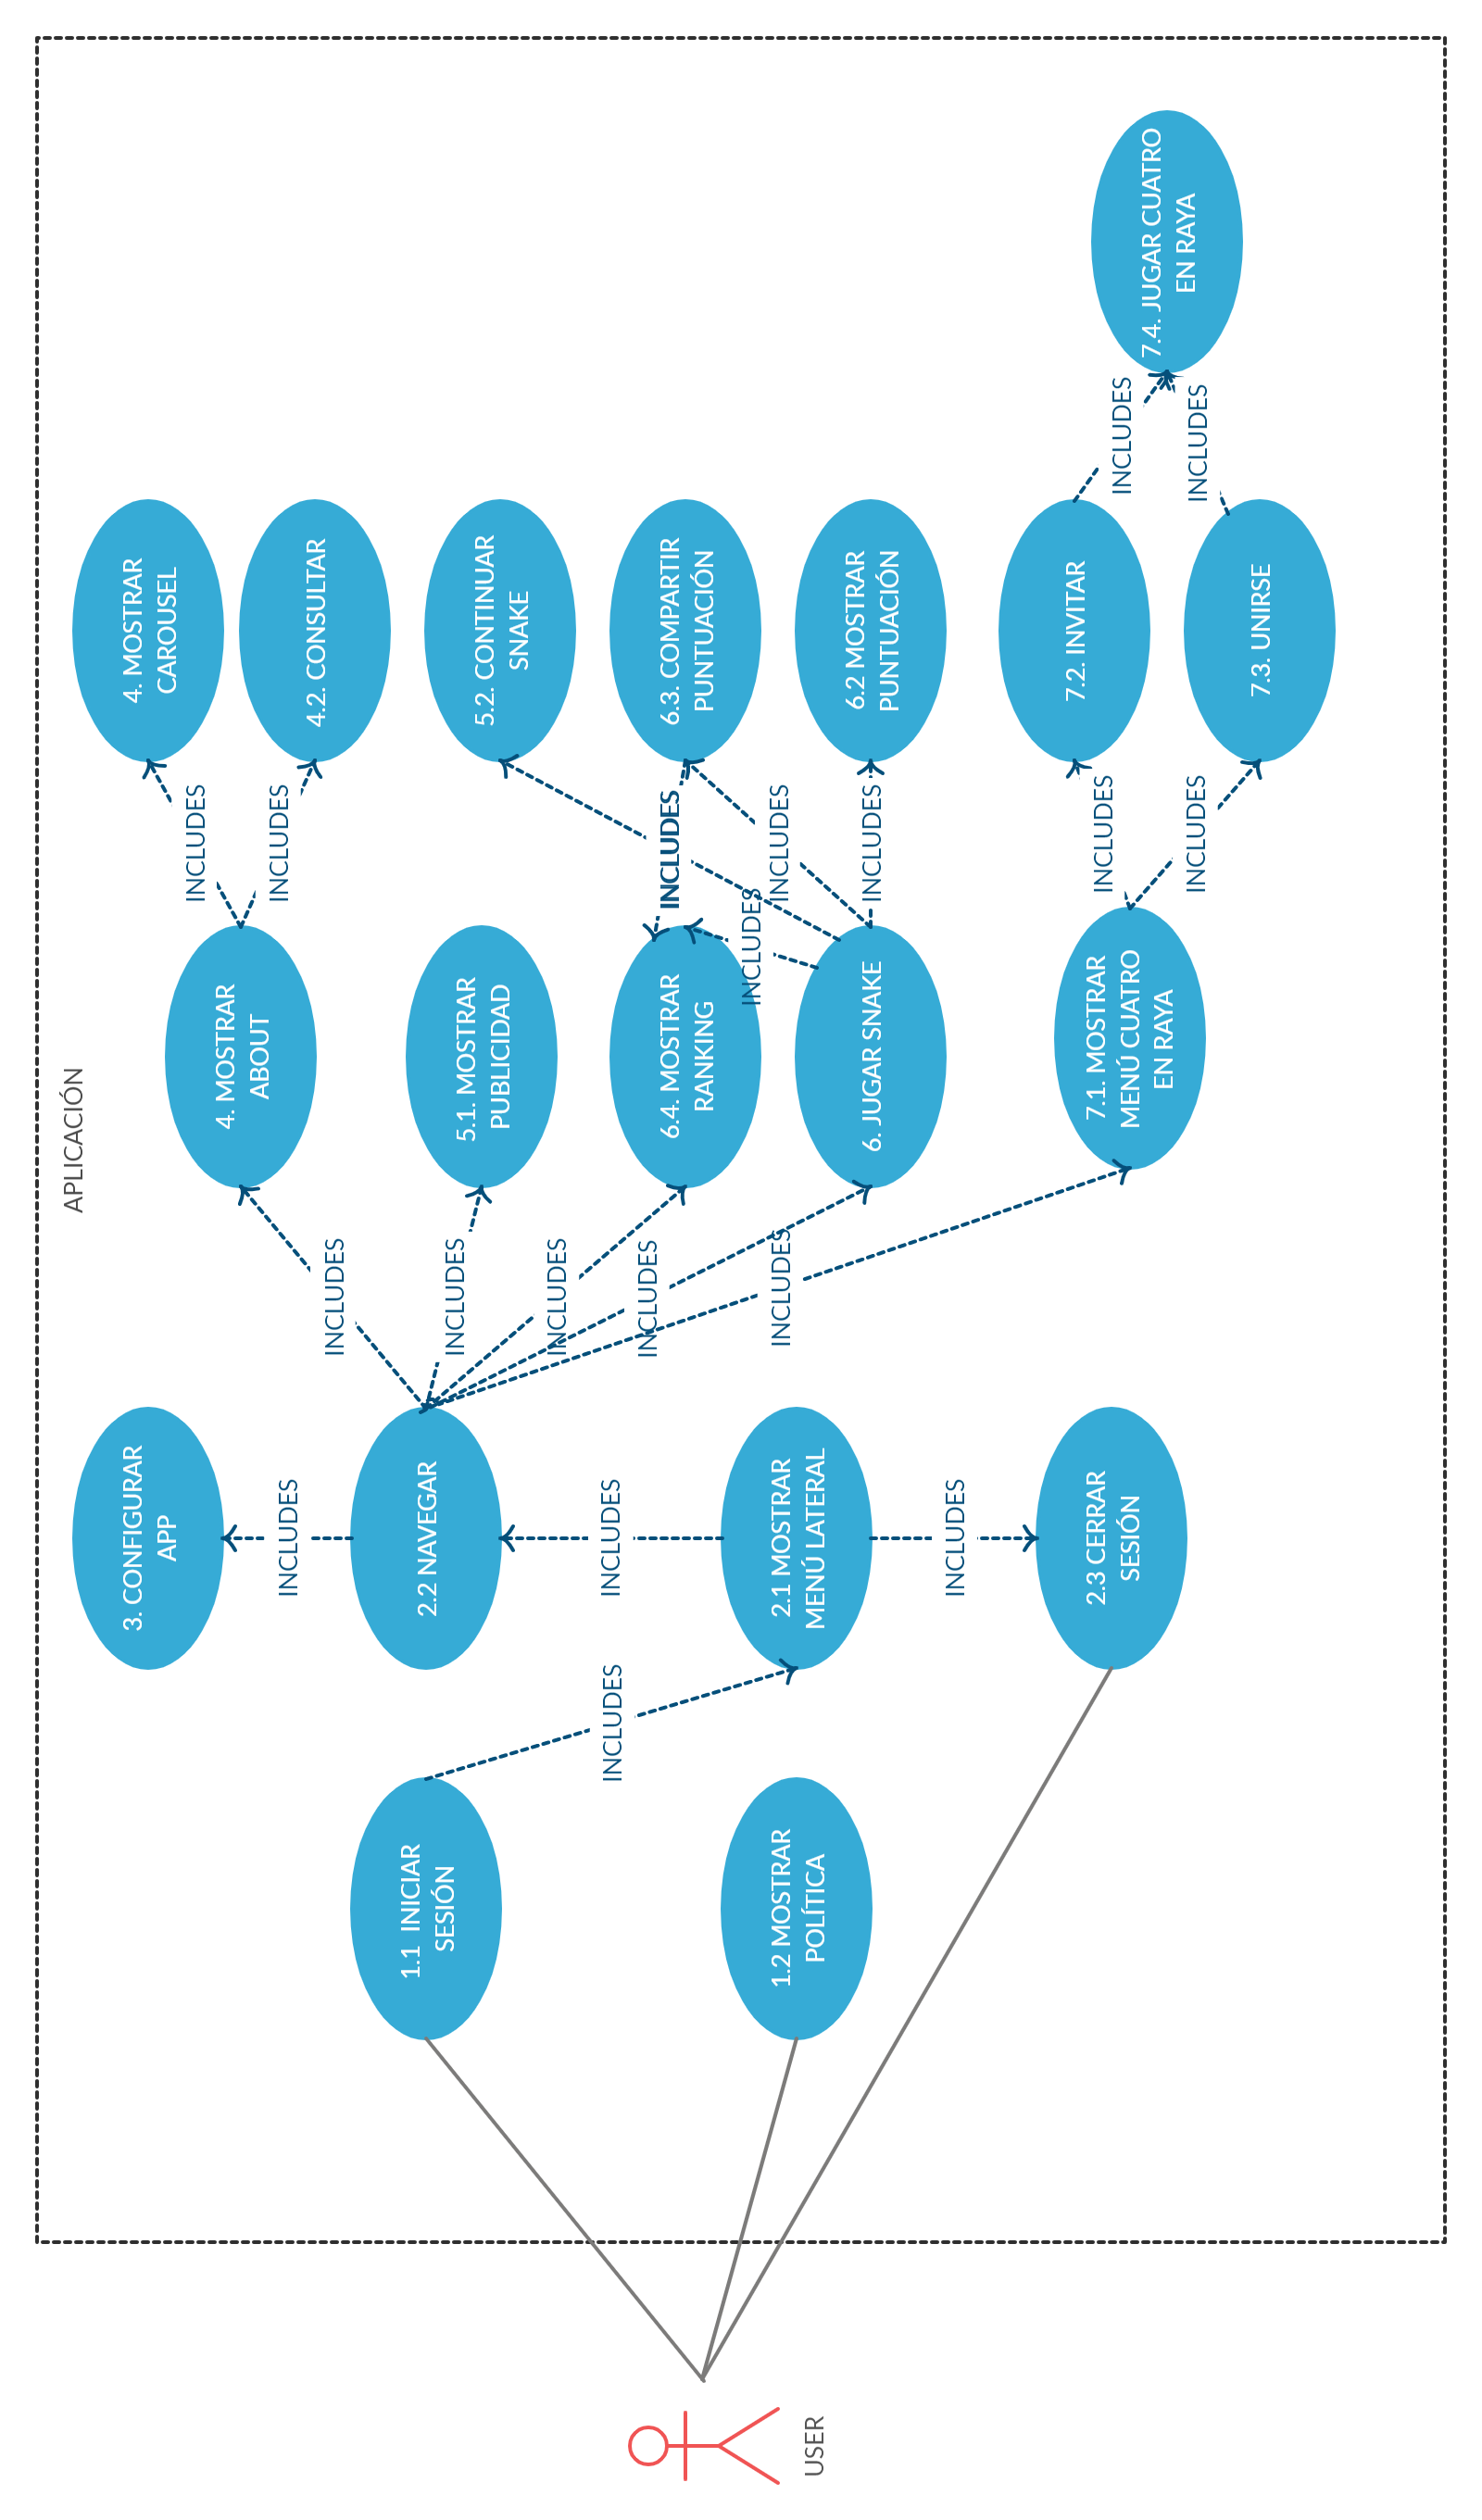
\includegraphics[width=0.93\textwidth]{requisitos/diagramauso.png}
	\caption{Diagrama con los casos de uso}\label{fig:diagramausp}
\end{figure}

\subsection{Casos de uso}

%%CASO DE USO PARA EL INICIO DE LA SESIÓN
\tablaSmallSinColores{Caso de uso 1: Sign in}{p{3cm} p{.75cm} p{9.5cm}}{tablaUC0}{
	\multicolumn{3}{l}{Caso de uso 1: Sign in} \\
}
{
	Descripción                            & \multicolumn{2}{p{10.25cm}}{Permite al usuario acceder a la aplicación mediante su cuenta de Google. Como consultar la política de privacidad.} \\\hline
	Requisitos                         	   & \multicolumn{2}{p{10.25cm}}{RF-1,RF-1.1,RF-1.2} \\\cline{1-3}Precondiciones                         &  \multicolumn{2}{p{10.25cm}}{Tener la aplicación descargada en el terminal}   \\\hline
	\multirow{2}{3.5cm}{Secuencia normal}  & Paso & Acción \\\cline{2-3}
	& 1    & EL usuario clicka en 'Privacy policy'.
	\\\cline{2-3}
	& 2    & Se muestra el navegador con lo política.
	\\\cline{2-3}
	& 3    & Se pulsa en el botón de 'Sign in'.
	\\\cline{2-3}
	& 4    & Se indica que cuenta de Google usar, entrando dentro de la aplicación.
	\\\hline
	Postcondiciones                        & \multicolumn{2}{p{10.25cm}}{Ninguna.} \\\hline
	Excepciones                        & \multicolumn{2}{p{10.25cm}}{No disponer de cuenta de Google}\\\hline
	Importancia                            & Alta \\\hline
	Urgencia                               & Alta \\\hline
	Frecuencia                               & Alta \\
}

%% CASO DE USO PARA MOSTRAR EL CONTENIDO DEL MENÚ
\tablaSmallSinColores{Caso de uso 2: Mostrar el menú}{p{3cm} p{.75cm} p{9.5cm}}{tablaUC0}{
	\multicolumn{3}{l}{Caso de uso 2: Mostrar el menú} \\
}
{
	Descripción                            & \multicolumn{2}{p{10.25cm}}{Da la capacidad al usuario de navegar entre las ventanas de la aplicación, como salir de la misma en el caso de que así lo requiera.} \\\hline
	Requisitos                         	   & \multicolumn{2}{p{10.25cm}}{RF-2,RF-2.1,RF-2.2,RF-2.3,RF-1.3} \\\cline{1-3}
	Precondiciones                         &  \multicolumn{2}{p{10.25cm}}{Haber realizado el requsito funcional primero.}   \\\hline
	\multirow{2}{3.5cm}{Secuencia normal}  & Paso & Acción \\\cline{2-3}
	& 1    & Deslizamiento horizontal derecho o pulsación en la hamburguesa, para mostrar el menú lateral.
	\\\cline{2-3}
	& 2    & Elegimos una de las diferentes opciones del menú.
	\\\cline{2-3}
	& 3    & Navegamos a la ventana escogida o salimos de la aplicación.
	\\\hline
	Postcondiciones                        & \multicolumn{2}{p{10.25cm}}{Ninguna.} \\\hline
	Excepciones                        & \multicolumn{2}{p{10.25cm}}{El menú no se encuentra disponible dentro de los juegos}\\\hline
	Importancia                            & Alta \\\hline
	Urgencia                               & Alta \\\hline
	Frecuencia                               & Alta \\
}

%%CASO DE USO PARA LA CONFIGURACIÓN DE LA APLICACIÓN
\tablaSmallSinColores{Caso de uso 3: Configuración de la aplicación}{p{3cm} p{.75cm} p{9.5cm}}{tablaUC0}{
\multicolumn{3}{l}{Caso de uso 3: Configuración de la aplicación} \\
}
{
Descripción                            & \multicolumn{2}{p{10.25cm}}{Dotar al usuario de las herramientas necesarias para poder hacer cambios de alguna de las partes del sistema.} \\\hline
Requisitos                         	   & \multicolumn{2}{p{10.25cm}}{RF-3,RF-3.1,RF-3.2} \\\cline{1-3}
Precondiciones                         &  \multicolumn{2}{p{10.25cm}}{Haber realizado el requisito funcional uno.}   \\\hline
\multirow{2}{3.5cm}{Secuencia normal}  & Paso & Acción \\\cline{2-3}
& 1    & Escoger del menú lateral la parte de 'settings'.
\\\cline{2-3}
& 2    & Una vez dentro, usar los 'sliders' activar o desactivar las funciones indicadas.
\\\hline
Postcondiciones                        & \multicolumn{2}{p{10.25cm}}{Ver que los cambios se producen.} \\\hline
Excepciones                        & \multicolumn{2}{p{10.25cm}}{Ninguna.}\\\hline
Importancia                            & Media \\\hline
Urgencia                               & Media \\\hline
Frecuencia                               & Alta \\
}

%%CASO DE USO PARA MOSTRAR EL CONTENIDO SOBRE EL CREADOR DE LA APLICACIIÓN
\tablaSmallSinColores{Caso de uso 4: Mostrar el contenido de About}{p{3cm} p{.75cm} p{9.5cm}}{tablaUC0}{
	\multicolumn{3}{l}{Caso de uso 4: Mostrar el contenido de about} \\
}
{
	Descripción                            & \multicolumn{2}{p{10.25cm}}{Disponer de la opción de ver quien es el creador de la aplicación y navegar a recursos.} \\\hline
	Requisitos                         	   & \multicolumn{2}{p{10.25cm}}{RF-3,RF-3.1,RF-3.2} \\\cline{1-3}
	Precondiciones                         &  \multicolumn{2}{p{10.25cm}}{Haber realizado el requisito funcional uno.}   \\\hline
	\multirow{2}{3.5cm}{Secuencia normal}  & Paso & Acción \\\cline{2-3}
	& 1    & Escoger del menú lateral la parte de 'About me'.
	\\\cline{2-3}
	& 2    & Pulsar en los 'iconbuttons' para mostrar el contenido seleccionado en el navegador. En el caso el botón sea de correo, nos tiene que abrir la aplicación correspondiente para mandar un feedback.
	\\\hline
	Postcondiciones                        & \multicolumn{2}{p{10.25cm}}{Ninguna.} \\\hline
	Excepciones                        & \multicolumn{2}{p{10.25cm}}{Ninguna.}\\\hline
	Importancia                            & Baja \\\hline
	Urgencia                               & Baja \\\hline
	Frecuencia                             & Baja \\
}